\documentclass[a4, 14pt]{extarticle}
\usepackage[dvipsnames]{xcolor}
\usepackage{pagecolor}
\usepackage{graphicx}
\usepackage{lipsum} 
\usepackage{hyperref}
\usepackage{amsmath,amssymb,amsfonts}
\usepackage[nameinlink]{cleveref}

\DeclareMathOperator*{\argmax}{arg\,max}
\DeclareMathOperator*{\argmin}{arg\,min}

\pagecolor{black}
\color{White}

\title{eBalo BlackPaper}
\author{Black Pepper Team}
\date{22 March 2024}

\begin{document}


\makeatletter
    \begin{titlepage}
        \begin{center}
            
\includegraphics[width=0.3\linewidth]{images/logo.png}\\[4ex]
            {\Huge \bfseries  \@title }\\[2ex] 
            { \Large \textit{\@author} } \\[5ex]
            {\textbf{Abstract}}\\
            \begin{flushleft}\small We introduce the novel way to manage your account through biometrics. Based on \textit{Iden3} technology, advanced \textit{Deep Learning} algorithms, we accomplished to create unique identities based on three types of biometrics: Face, Voice, and Passport Data, although the system is easily extended to more types of biometrical data. Additionally, we extend the protocol to include functionality of transferring funds solely based on the person's photo, as long as he is registered in the protocol as well.
            \end{flushleft}
            \\[20ex]
            {\large \@date}
        \end{center}
    \end{titlepage}
\makeatother
\thispagestyle{empty}
\newpage

%Add content for page two here (useful for two-sided printing)
\newpage

\section{Introduction}

We propose an innovative approach to account management leveraging biometric data. Powered by cutting-edge Iden3 technology and sophisticated Deep Learning algorithms, we've achieved the creation of distinctive identities based on three key biometric modalities: Facial recognition, Voice recognition, and Passport data. Moreover, our system boasts seamless scalability to incorporate additional biometric data types. Excitingly, we're enhancing the protocol to enable fund transfers exclusively through a person's photograph, provided they're registered within the system.

To achieve our goals, we heavily rely on Account Abstraction. The existing limitations preclude innovation in a number of important areas, particularly:
\begin{itemize}
    \item Smart contract wallets that use signature verification other than ECDSA (eg. Schnorr, BLS, post-quantum etc.)
    \item Smart contract wallets that include features such as multisig verification or social recovery, reducing the highly prevalent risk of funds being lost or stolen
    \item Privacy-preserving systems like $\mathsf{tornado.cash}$
    \item Users being able to pay for transaction fees in a token other than ETH (e.g. by converting that token into the ETH needed for fees inside the transaction in real-time)
\end{itemize}

By employing both Account Abstraction with the deep learning biometric authorization techniques, we are able to combine the convenience of both. In the subsequent sections, we dwelve into exploring how our system works precisely.

\section{Main Flow}
In this section, we describe three main flows:
\begin{itemize}
    \item Saving Biometrics in Registry, which is described in \Cref{flow:getting_id}.
    \item Account Registration, explained in \Cref{flow:registration}.
    \item Paying using someone's biometrics, which is described in \Cref{flow:paying}.
    \item Recovering your keys, which is described in \Cref{flow:recovery}.
\end{itemize}

\subsection{Saving Biometrics in Registry}\label{flow:getting_id}

The procedure for saving biometric data in a registry encompasses multiple phases, beginning with the initial interaction by the user and concluding with the definitive storage of data. During this process, the user's biometric data is validated by dedicated issuers, and a snapshot of it is stored on-chain.

\textbf{User Submission}: The initiation of the process involves the user approaching the issuer and submitting their biometric data. This data may include facial recognition details, voice samples, video snippets, or other biometric identifiers.

\textbf{Validation}: Following the data submission, the issuer undertakes necessary validations of the biometric data, ensuring the user's uniqueness.

\textbf{Claim Creation}: After the data validation, the issuer issues a claim to the user with their biometric data. The further connection of the user account and user biometrics is done by the user themselves, as explained in the \Cref{flow:registration}.

\textbf{State Transition}: After the user's claim issuance, the issuer transitions state on-chain; in addition to regular state transition proof and data, an array of Biometric Data structures are transitioned by the issuer as well. The Biometric Data structure contains the following fields:

\begin{itemize}
    \item A unique identifier (\texttt{uuid}) linking the user to their biometric particulars,
    \item The Ethereum address of the user (aka administrator address), signifying ownership of the Smart Account,
    \item The raw biometric data, and
    \item Supplementary metadata pertinent to the user.
\end{itemize}

The whole process is illustrated in \Cref{fig:registration}.

\begin{figure}
    \centering
    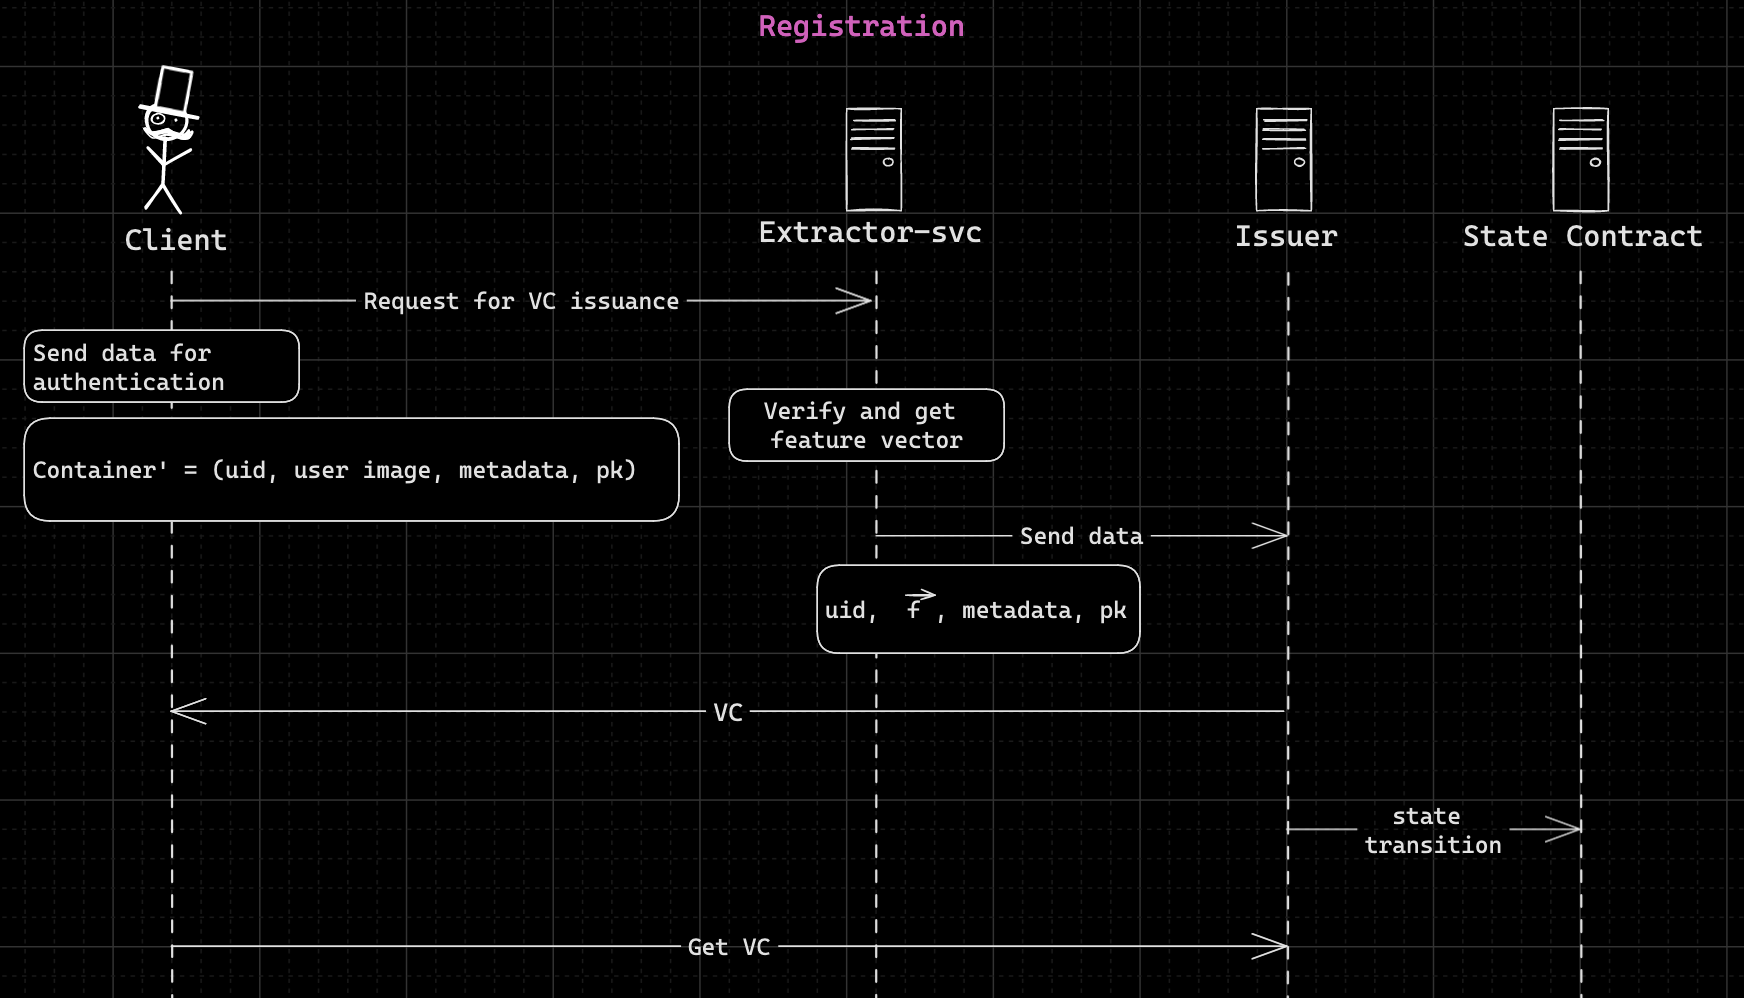
\includegraphics[width=\textwidth]{images/registration_flow-modified.png}
    \caption{Registration flow}
    \label{fig:registration}
\end{figure}

\textbf{Security and Access}: As soon as at least one issuer transitions the user's data, the user can proceed with Smart Account creation, allowing them to interact with the Blockchain ecosystem. In the following sections, \Cref{flow:paying} and \Cref{flow:recovery}, we will dive deeper into the functionality of the Smart Account.

\subsection{Account Registration}\label{flow:registration}

After the state is transitioned by the issuer, the user is able to prove to the issuer that they "hold" the correct biometrics. To create an account, the user proves that a trusted issuer (by the user themselves) transitioned a state, and recorded addresses on-chain, and that they hold a private keys for those addresses.

After the Smart Account is created, the user uses their biometrics and knowledge of the address provided with the biometric; they pass to the issuer an address of the Smart Account. The issuer uses the provided data to connect the User's Biometrics, EOA, and the Smart Account address, allowing fast account recovery in case the keys to the administrator address are lost.

\subsection{Paying through Biometrics}\label{flow:paying}

After the Smart Account is created, the user can fund it and interact with the ecosystem where the SA is deployed. 

The main requirement for the user, each time they want to send money or interact with the contract, is to prove that $k$ of $n$ issuers issued a claim and transitioned data with the addresses to which they know the private keys. The process is illustrated in \Cref{fig:transfer}.

\begin{figure}
    \centering
    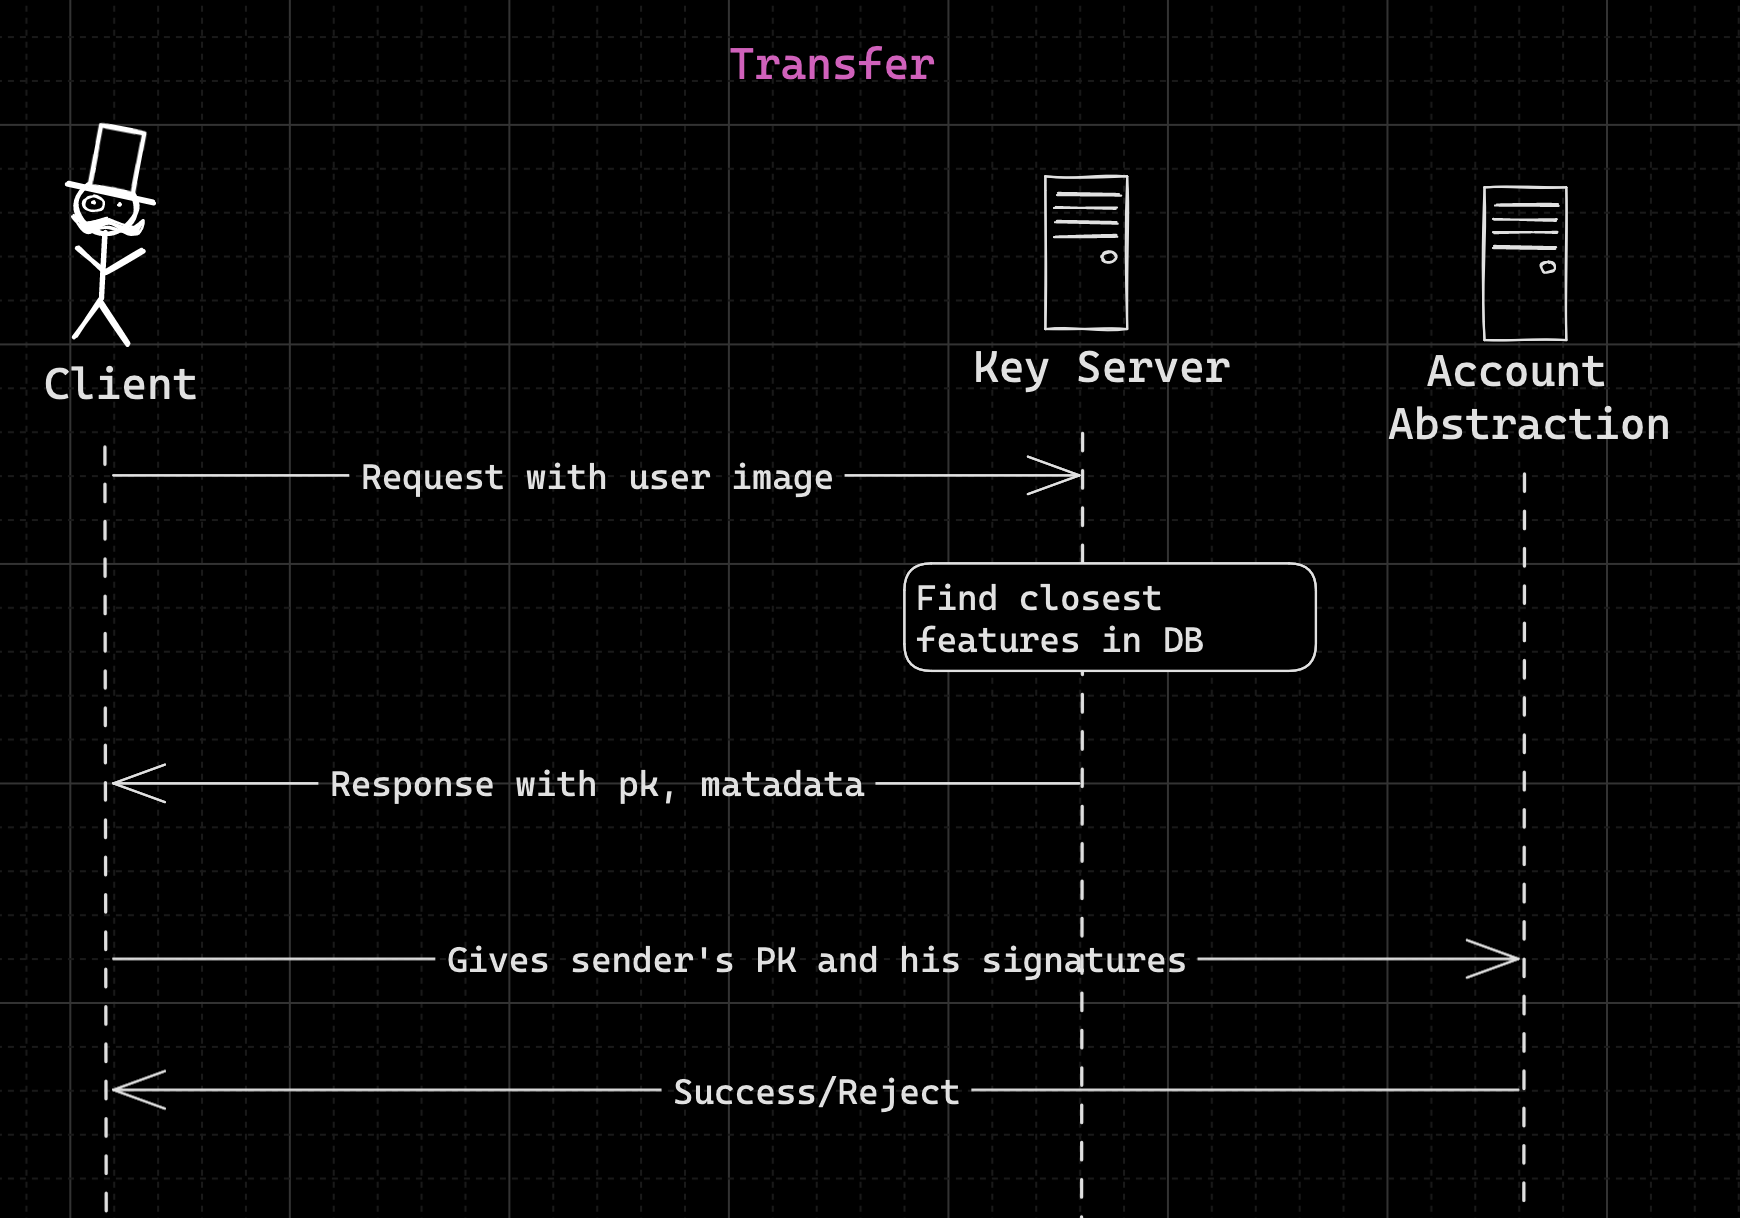
\includegraphics[width=\textwidth]{images/transfer_flow-modified.png}
    \caption{Transferring flow}
    \label{fig:transfer}
\end{figure}

\subsection{Identity Recovery}\label{flow:recovery}

In case the user loses access to the EOA that manages the Smart Account, they can provide to the trusted issuers their new biometric data and addresses, and an address of the Smart Account. Based on this information, the issuer revokes previous claims to the user, and transitions a new state and changes the addresses of the administrator accounts. The process is illustrated in \Cref{fig:recovery}.

\begin{figure}
    \centering
    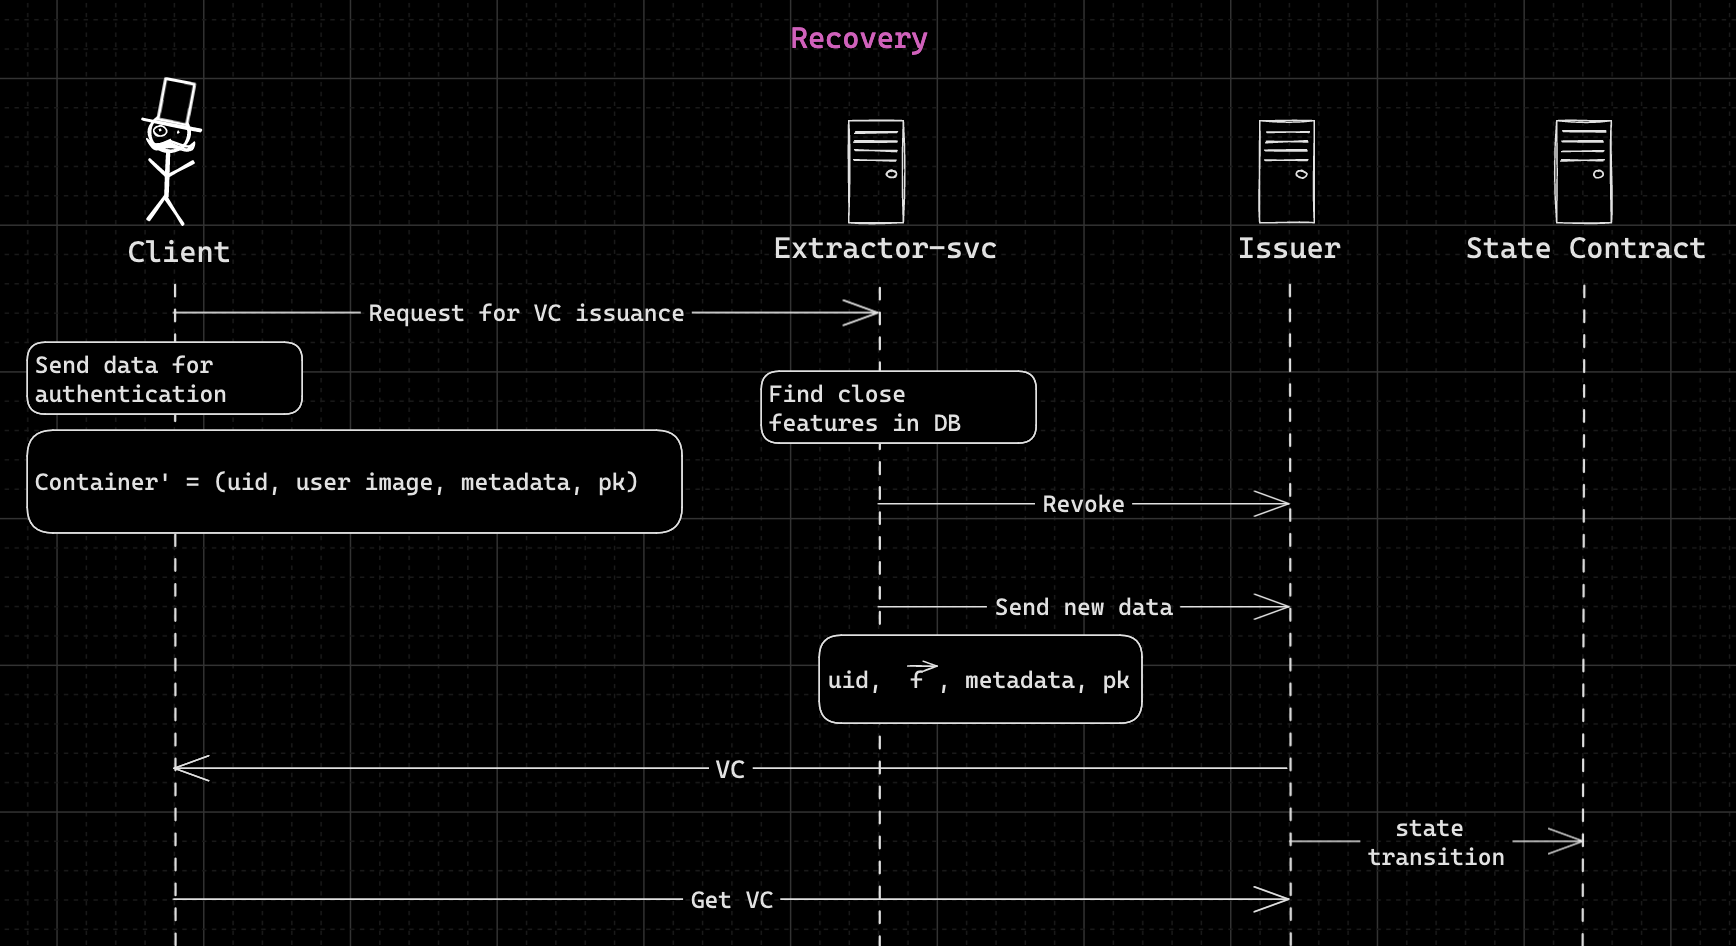
\includegraphics[width=\textwidth]{images/recovery_flow-modified.png}
    \caption{Recovery flow}
    \label{fig:recovery}
\end{figure}

\section{Artificial Intelligence: how and why?}
However, the question remains: how can we effectively compare two photo images? Historically, there are various approaches how to handle this problem. In \Cref{ai:classical} we are going to overview the classical approaches to face image analysis, in \Cref{ai:deep} we describe the state-of-the-art deep learning-based method we employed, while finally in \Cref{ai:voice} we briefly explain certain aspects of voice recognition. The curious reader might additionally read the \Cref{ai:details}, which explains the mathematics behind training such neural networks.

\subsection{Classical Approaches to Facial Analysis}\label{ai:classical}
Traditionally, there exist many traditional methods, including:
\begin{itemize}
    \item \textit{Eigenface} \cite{eigenface}: assuming that every face is made of lots of ``custom'' face images overlaid on top of each other, we recognize an unknown image by working out which Eigenfaces it is likely composed of (see \Cref{fig:eigenface} for details). However, the Eigenface is super sensitive to any kind of noise, and therefore is obsolete in terms of accuracy.
    \item \textit{Facial Feature Points} \cite{wang2014facial}: finding key points on the face image, see \Cref{fig:face-features} for illustration. To compare two faces, one compares corresponding key points. Similarly to \textit{Eigenface}, this approach heavily relies on the fact that the face is perfectly aligned and the illumination is sufficient to see the whole face.
\end{itemize}

\begin{figure}
    \centering
    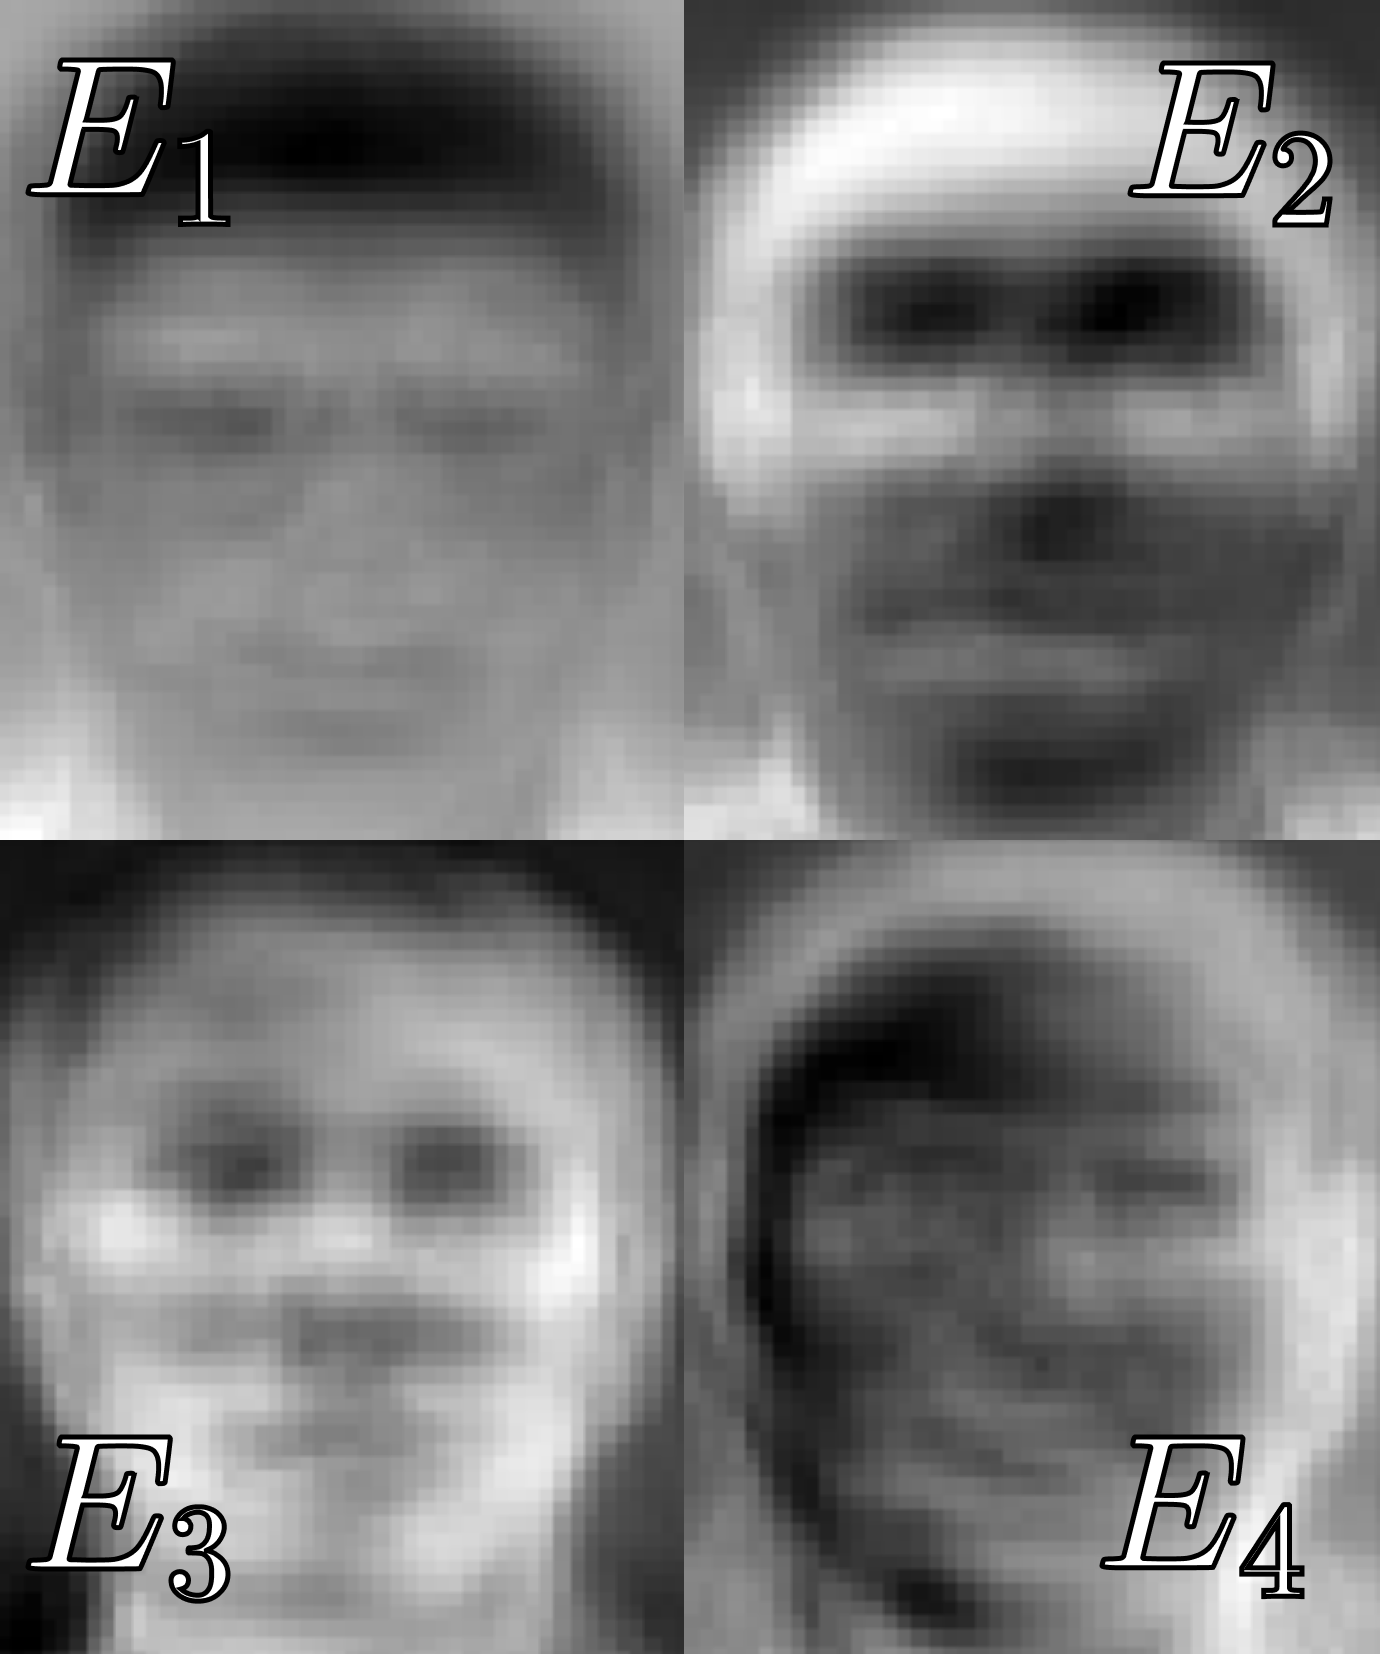
\includegraphics[width=0.5\textwidth]{images/eigenface.png}
    \caption{A set of predetermined Eigenfaces $\{E_i\}$. The main assumption that each face $P$ can be viewed as a composition of all $E_i$ with certain corresponding proportions (aka, the linear combination).}
    \label{fig:eigenface}
\end{figure}

\begin{figure}
    \centering
    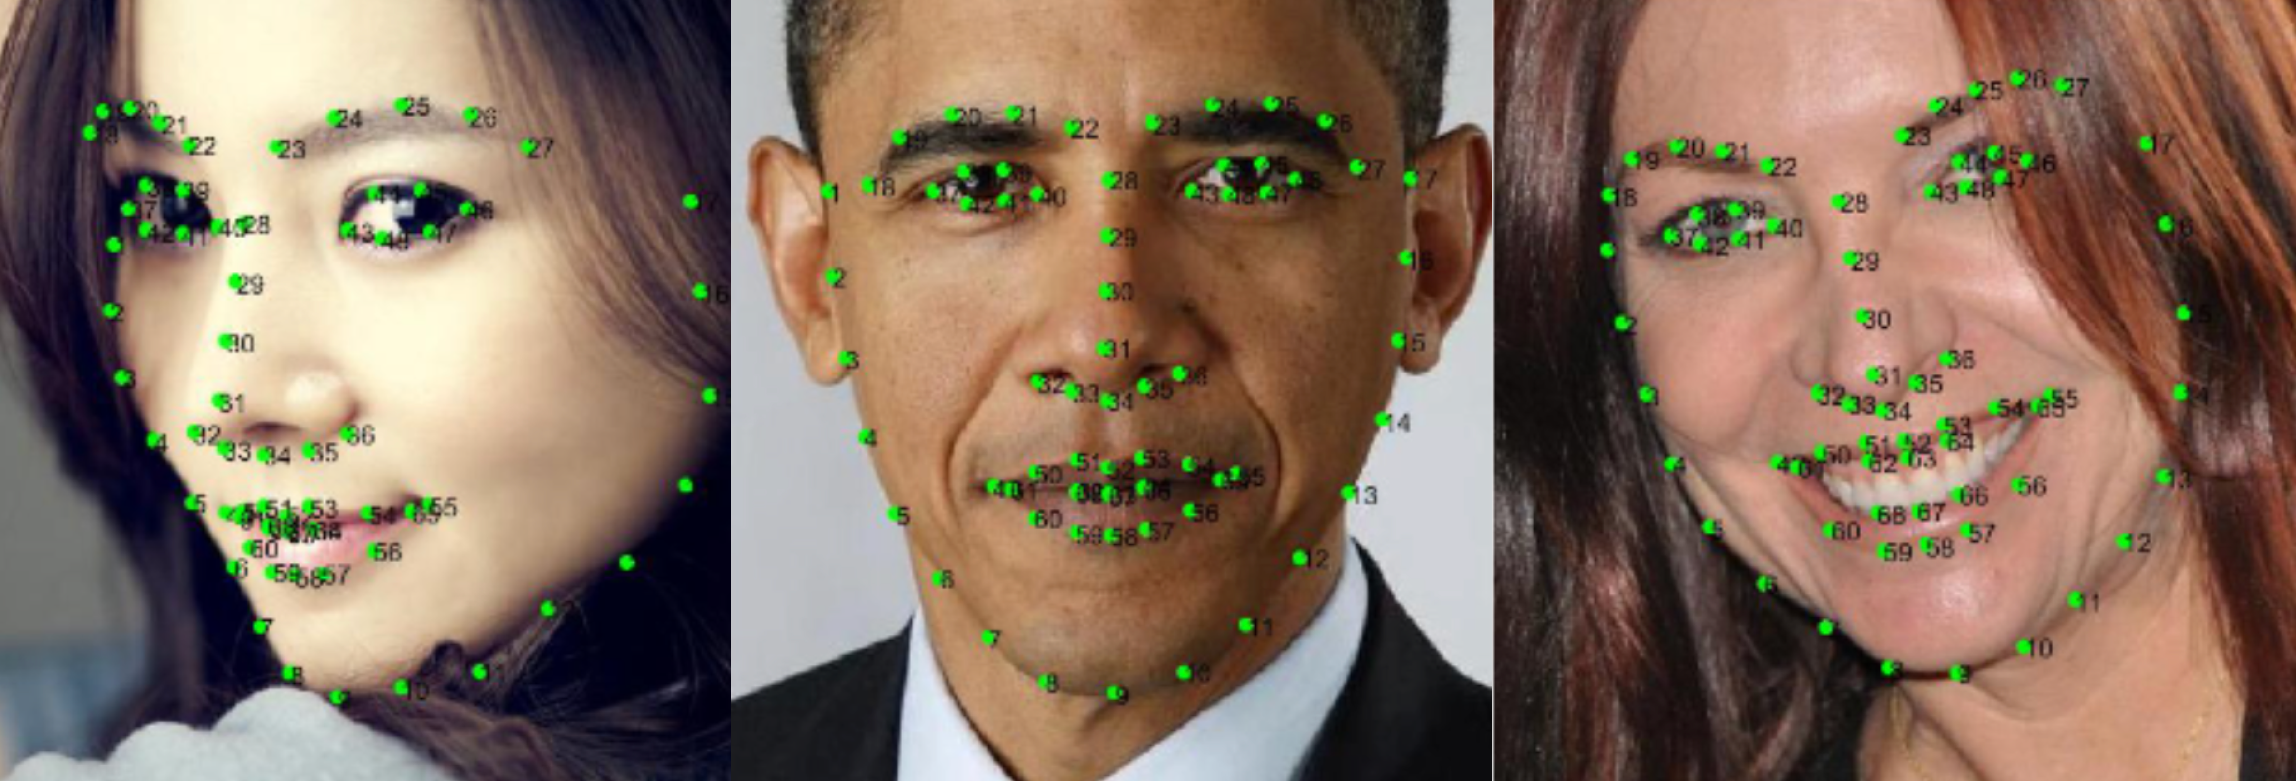
\includegraphics[width=0.8\textwidth]{images/face_features.png}
    \caption{Facial Feature Points approach: the mathematical model is able to detect key points and two people can effectively be compared using them.}
    \label{fig:face-features}
\end{figure}

To eliminate these inaccuracies, approximately in 2014-2015, the signficant breakout happened that allow to use neural networks to perform the analysis: namely, the \textit{FaceNet} paper \cite{Schroff_2015}.

\subsection{Deep Learning-based Approach}\label{ai:deep}

The core idea is pretty straightforward: instead of operating with the image directly, we transform it to the vector of fixed size $n$. Denote the set of images by $\mathcal{I}$. Our goal is to build a map $\mathcal{I} \mapsto (x_1,\dots,x_n)$. In our particular case, $n=128$, that is we get $128$ different real numbers as an output, called \textit{embeddings}. These vectors are depicted in \Cref{fig:sphere}.

\begin{figure}
    \centering
    \includegraphics[width=0.5\textwidth]{images/feature_vectors.png}
    \caption{Each person's photo produces a ``similar'' set of numbers $(x_1,\dots,x_n)$, which, if viewed geometrically, are located close in space.}
    \label{fig:sphere}
\end{figure}

To parameterize such a model, one employs the Convolutional Neural Networks (CNNs) \cite{oshea2015introduction}, which can learn super intricate and incredibly complex data behaviour and patterns. 

Now, how do we compare two face images $X,Y \in \mathcal{I}$? We first find embeddings of $X$ and $Y$, say, $\boldsymbol{f}_X$ and $\boldsymbol{f}_Y$, respectively, and then compare the distances between them as follows:
\begin{equation}
    d(X,Y) = \sum_{i=1}^n (f_X^{\langle i \rangle} - f_Y^{\langle i \rangle})^2,
\end{equation}
where $f^{\langle i \rangle}$ denotes the $i^{\text{th}}$ component in vector $\boldsymbol{f}$. If this distance is small enough (technically, less then a certain constant \textit{threshold} $\tau$), $X$ and $Y$ are perceived to be of the same identity.

This way, the issuer can store the correspondence between the certain identity and the feature vector in the local database. When some user logins, the issuer computes his feature vector $\boldsymbol{f}'$ and compares it to every feature vector $\boldsymbol{f}$ in the database. The smallest $d(\boldsymbol{f},\boldsymbol{f}')$ which is below the threshold, is the identity $\boldsymbol{f}'$ belongs to. 

One additional essential note is whether it is safe to store $\boldsymbol{f}$ directly in the database, that is, can the attacker produce the pre-image of vector $(x_1,\dots,x_n)$? Although not proven, it is practically incredibly hard to accomplish, even for widely recognized \textit{FaceNet}. Indeed, knowing the key points, for example, can you fully restore the original image? This problem is highly underconstrained and therefore difficult to solve. 

\subsubsection{Effective feature vector storage}
Since the derived features are further stored on-chain, it is crucial to optimize the memory space needed to store a single feature vector $\boldsymbol{f}$. For that reason, we propose to use a quite simple transformation:
\begin{equation}
    x_i \mapsto [\alpha \cdot x_i + \beta],
\end{equation}
where $[\cdot]$ is a flooring operation. The bigger $\alpha$ is, the better accuracy is obtained, yet more space is needed to store the vector. Practically, even for $\alpha \approx 100$, the accuracy drop is insignificant. 

Besides, in the majority of neural networks, the output is \textit{normalized} -- meaning, that all $x_i$ are between $-1$ and $1$. For that reason, if $\beta$ is set to $1$ and $\alpha < 127$, instead of storing an array of $\mathsf{double}$'s, we use an array of $\mathsf{uint8}$'s. 

The best (in terms of memory space) approach is to \textit{binarize} the vector, which can be done simply as:
\begin{equation}
    x_i \mapsto \begin{cases}
        1, & x_i \geq 0 \\
        0, & x_i < 0
    \end{cases}
\end{equation}
This would make each vector weigh only $n$ bits (in our case, $128$ bits). However, that results in a significant drop of accuracy, so we decided not to use it. In turn, choosing $\alpha=127$ and $\beta=1$ allows to reduce the cost for storing feature vectors while achieving a decently high accuracy.


\subsection{Voice Recognition}\label{ai:voice}

In our implementation, we use the state-of-the-art \textit{Speechbrain}\cite{ravanelli2021speechbrain} technology, which gives us both \textit{Speaker Identification} and \textit{Voice Recognition} solutions. The idea of this neural network is similar to previously considered, but here, the data is \textit{sequential}: namely, the waveform data. That means, that instead of using CNNs, the Recurrent Neural Networks are used or even more advanced methods like Self-Attentional Mechanisms etc. The curious reader is directed to \cite{bai2021speaker}, but the core idea is the same: after the voice processing, we get the feature vector, but in this case consisting of $40000$ elements. 

\subsection{Technical Details: How to Train?}\label{ai:details}
\textit{Note:} This section is optional and not neccesary for understanding the flow, however is neccessary for building custom verification nets.

Denote by $\mathcal{B}$ a set of biometrics we are going to use (for example, for an RGB image we have $\mathcal{B} = \mathbb{R}^{W \times H \times n_C}$). 

Now, we form the dataset $\mathbb{T} = \{(p^{\langle i \rangle},p^{\langle i \rangle}_+,p^{\langle i \rangle}_-)\}_{i=0}^{n_T} \subset \mathcal{B}^3$ where $p^{\langle i \rangle}$ and $p^{\langle i \rangle}_+$ belong to the same person (called \textit{anchor} and \textit{positive} images, respectively) while $p^{\langle i \rangle}_-$ to distinct people (called a \textit{negative} image). The idea of a triplet loss is to make embedding distance between anchor and negative larger than between anchor and positive. However, this condition on its own does not produce sufficiently good results, so we make an additional restriction: we want to have anchor-negative distance larger than an anchor-positive by a \textit{margin} $\gamma \in \mathbb{R}_{\geq 0}$. That being said, ideally, for any $(p,p_+,p_i) \in \mathbb{T}$ we want:
\begin{equation}
\gamma + d_E(p,p_+) < d_E(p,p_-).
\end{equation}
Formally speaking, suppose that we sample triplets $T=(p,p_+,p_-)$ from a true data distribution $\rho_{\text{data}}$. Our goal is to find such embedding model $E^*$ that maximizes the probability of the previously mentioned relationship:
\begin{equation}
    E^* = \argmax_{E}\mathbb{P}_{\langle p,p_+,p_- \rangle \sim \rho_{\text{data}}}\left[\gamma+d_{E}(p,p_+) < d_{E}(p,p_-) \right]
\end{equation}
Since this task is complicated to be directly solved, instead one considers the \textit{triplet loss function} to be minimized:
\begin{equation}\label{eq:triplet_loss}
\mathcal{L}_{\text{triplet}}(E)\triangleq \mathbb{E}_{\langle p,p_+,p_- \rangle \sim \rho_{\text{data}}}\left[\text{ReLU}\left(d_{E}(p,p_+) - d_{E}(p,p_-) + \gamma\right)\right],
\end{equation}
and thus we choose $E^*=\argmin_E \mathcal{L}_{\text{triplet}}(E)$.

\small
\bibliographystyle{alpha}
\bibliography{refs}

\end{document}